\section{Introduction}
  In~\autoref{chap:preliminaries}, we have explained why finding numerical
  representations of words, called \textit{word embeddings}, can help
  downstream models that use them to solve NLP tasks. Word embeddings can also
  be used as a starting point for more complex models. The structure of the
  embedding vector space should reflect the linguistic information and
  properties of words so that downstream fine-tuned models can learn about the
  relations between words and make better predictions. Therefore, word
  embeddings should be ``good'' representations of the language in order to be
  helpful for the downstream models using them.\medskip

  The notion of ``good'' word representations is vague, so let us define what
  good word embeddings mean. A ``good'' word embedding is able to encode
  relations and linguistic properties of words. First, semantic information
  about the meaning of words should be present within word embeddings. For
  example, it needs to encode that a keyboard is more related to a computer than
  to a spoon. Second, syntactic information should also be present: word
  embeddings should encode that verbs are different from nouns or adverbs.
  Third, relations between words also need to be encoded, such as the relation
  between a country and its capital city or the relation between masculine nouns
  and their femininine equivalent. Lastly, ``good'' word representations should
  give good performances when they are used into another model to solve a NLP
  task. We can measure how good is the encoded linguistic information in word
  embedding with evaluation tasks, like intrinsic or extrinsic evaluations
  (see~\autoref{ch01:sec:word-embeddings-evaluation}
  in~\autoref{chap:preliminaries}). Intrinsic evaluations measure how much
  linguistic information is encoded in word embeddings while extrinsic
  evaluations measure how useful are the embeddings when they are used by
  downstream models.\medskip

  Finding ``good'' word representations is a difficult problem because
  linguistic information can be of different nature (semantic, syntactic) and
  the vector space of word embeddings is infinite so there are no perfect
  representations nor a unique solution to this problem. Seminal works on word
  vectors~\citep{osgood1964semantic, bierwisch1970classifying} tried to find the
  embeddings values manually by setting vector values with common information
  (like values indicating if a word belongs or not to a specific semantic
  group). But manually setting embeddings values is a complex and expensive task
  because the vocabulary size can be very large and the linguistic expertise
  required to know which information should be incorporated into word embeddings
  is costly and time-consuming. NLP scientists turned to machine learning
  algorithms and statistical models to automatically solve this problem and
  learn word embeddings. This chapter describes the most common models used to
  learn word representations and discusses the strenghts and weaknesses of each
  one.

\section{General methods to learn word embeddings}
  Different models have been created to learn word embeddings. They can be
  divided into three main categories:
  \begin{enumerate}
    \item statistical language modeling,
    \item neural network approaches,
    \item matrix factorization approaches.
  \end{enumerate}

  \noindent The three categories are described
  in~\autoref{ch03:subsec:statistical-language} for statistical language models,
  \autoref{ch03:subsec:neural-network} for neural networks and
  \autoref{ch03:subsec:matrix-factorization} for matrix factorization.

  \subsection{Statistical language modeling}
    \label{ch03:subsec:statistical-language}
    A statistical language model learns a probability distribution over all
    possible sentences of a language. It also learns the probability of a word
    to appear in a sentence if the previous words of the sentence are known.
    More formally, let $S$ be a sentence composed of $n$ words $S =
    w_1,~w_2,~\dots, ~w_k,~\dots, ~w_n$. A statistical language model learns the
    conditional probability that a word $w_i$ occurs given all the previous
    ones:

    \begin{equation}
      P(w_i~|~w_1,~w_2,~\dots,~w_{i-1})
    \end{equation}

    \noindent The model also learns the probability of each sentence $S$ with:

    \begin{equation}
      P(S) = P(w_1,~\dots,~w_n)
            = \prod_{i = 1}^n P(w_i~|~w_1,~\dots,~w_{i-1})
    \end{equation}

    \noindent These models are mostly used for speech
    recognition~\citep{bahl1989tree} or machine
    translation~\citep{brown1990statistical} because in those tasks words are
    processed sequentially and are strongly related to the ones already
    processed. A speech recognition system cannot use the next words of the
    sentence to predict the current one because they have not been spoken yet.
    Note here that it is different from a text classification system. In a
    classification system, all the words of the text are simultaneously
    available to the model to make its predictions.
    While statistical language modeling are able to encode linguistic
    information (some words are more related to others because their probability
    to appear in a given context is higher), it fails to model relations between
    words that are in consecutive sentences and have poor generalization
    properties (they are highly dependent on the training data).

  \subsection{Neural network approaches}
    \label{ch03:subsec:neural-network}
    \subsubsection{Seminal works}
      Statistical language modeling learns a probability distribution of
      sequences of words in a language. This probability distribution is learned
      over a large corpus of text. The model is then used to predict words of a
      sentence, \textit{e.g.} for language translation or speech recognition
      tasks. But sentences used for testing or for inference are likely to be
      different from sentences used during training because, for example, people
      want to translate texts that have not been translated yet. Therefore,
      learning a probability distribution that can generalize well on unseen
      sentences is a difficult task as the dimension of the probability
      distribution grows exponentially with the number of words in the
      vocabulary and the length of sequences.~\citeauthor{bengio2003neural}
      \citep{bengio2003neural} propose to solve this problem by learning a
      distributed representations of words.  They associate a $d$-dimensional
      vector $\mathbf{v}_w \in \mathbb{R}^d$ to each word $w$ of the vocabulary
      and learn simultaneously the probability distribution of word sequences as
      a function of those vectors. The dimension of the vector space is fixed
      and is no longer dependent on the vocabulary size or the lengths of
      sequences. The probability distribution is learned with a neural network
      architecture where the inputs are the word vectors of the sequence
      $w_1,~\dots,~w_{k-1}$ and the output is a vector whose $i$-th value is the
      probability that the word $w_i$ is the next word in the sequence. \medskip

      In~\citeyear{collobert2008unified},
      \citeauthor{collobert2008unified}~\citep{collobert2008unified} proposed a
      novel architecture that jointly learns representations of words and how to
      use them in different tasks. The model aims to solve simultaneously
      part-of-speech (POS) tagging, chunking, semantic role labeling, name
      entity recognition and predicting if two words are related or not with a
      multitask learning scheme. The model they use is a single convolutional
      neural network that takes a sentence as input and outputs a vector of
      probabilities of belonging to each possible class for a given NLP task.
      Since neural networks cannot handle inputs of variable size, the authors
      rely on the \textit{window approach} which consists in selecting and
      giving the network the $m$ words around the target word to classify.
      \autoref{ch03:fig:collobert2008} represents their model architecture. The
      output layer is dependent on the selected task to solve but the
      representations of words found in the lookup tables are shared for all the
      tasks. Word embeddings should therefore encode many different types of
      linguistic information and not only those required to solve a single
      specific task. During training, a single example from one of the tasks is
      selected and the parameters of the network are updated with the gradient
      descent on the loss of this example. While some labels help the model to
      learn (\textit{e.g.} to indicate the part-of-speech tag of words for the
      POS tagging task), there are no labels to help the model to know what the
      values of word embeddings should be. The model has to learn the values
      that best solve all the tasks. This type of learning is called
      \textbf{semi-supervised learning}
      (see~\autoref{ch02:subsec:semi-supervised-learning}
      in~\autoref{chap:preliminaries}). \medskip

      \begin{figure}[h!]
        \centering
        % 0.43\textwidth is the max size the image can have to stay on same page
        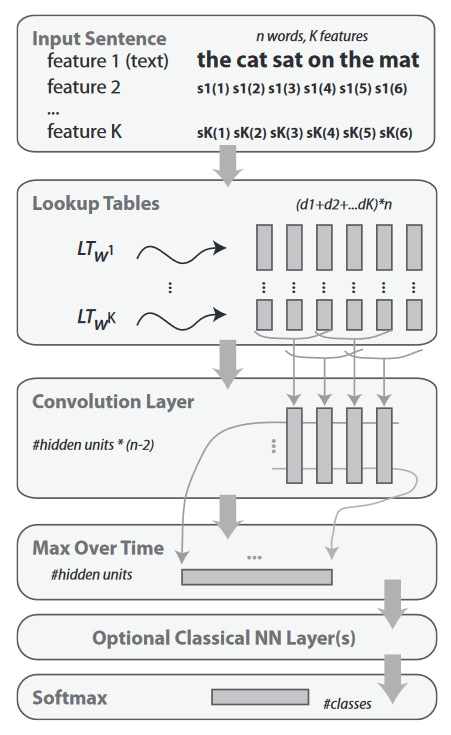
\includegraphics[width=0.43\textwidth]{ch03-collobert2008.png}
        \caption[Neural network used to learn word embeddings by
        \citeauthor{collobert2008unified}.] {The neural network architecture
        used to learn word representations in~\citep{collobert2008unified}.
        Word representations are fed into a convolutional layer to output a
        vector of probabilities of belonging to certain classes.}
        \label{ch03:fig:collobert2008}
      \end{figure}

      In~\citeyear{collobert2011natural},
      \citeauthor{collobert2011natural}~\citep{collobert2011natural} extended
      their neural network architecture to also feed the network with a complete
      sentence (\autoref{fig:collobert-sentence2011}), not only with a window of
      words (\autoref{fig:collobert-window2011}). The window approach was
      limiting the performance of the system in the semantic role labeling task
      because the information needed to correctly predict the answer is often
      outside the window. To feed the network with a
      sentence,~\citeauthor{collobert2011natural} start by using the lookup
      tables to get the embeddings of each word and then use some convolutions
      to get a vector of fixed size. This vector is then fowarded to hidden
      layers of the network to produce an output vector which is, like in the
      window approach method, composed of the probabilities to belong to each
      possible class for a given task.

      \begin{figure}[hb]
        \centering
        \begin{subfigure}[t]{0.49\textwidth}
          \centering
          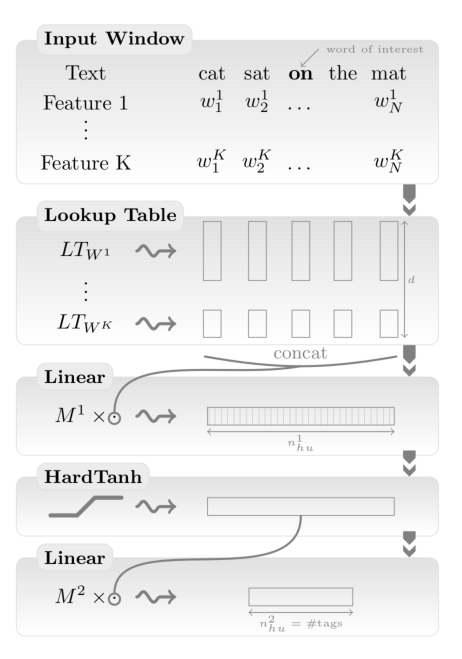
\includegraphics[width=0.72\textwidth]{ch03-collobert-window2011}
          \caption{Neural network with a window approach.}
          \label{fig:collobert-window2011}
        \end{subfigure} \hfill
        \begin{subfigure}[t]{0.49\textwidth}
          \centering
          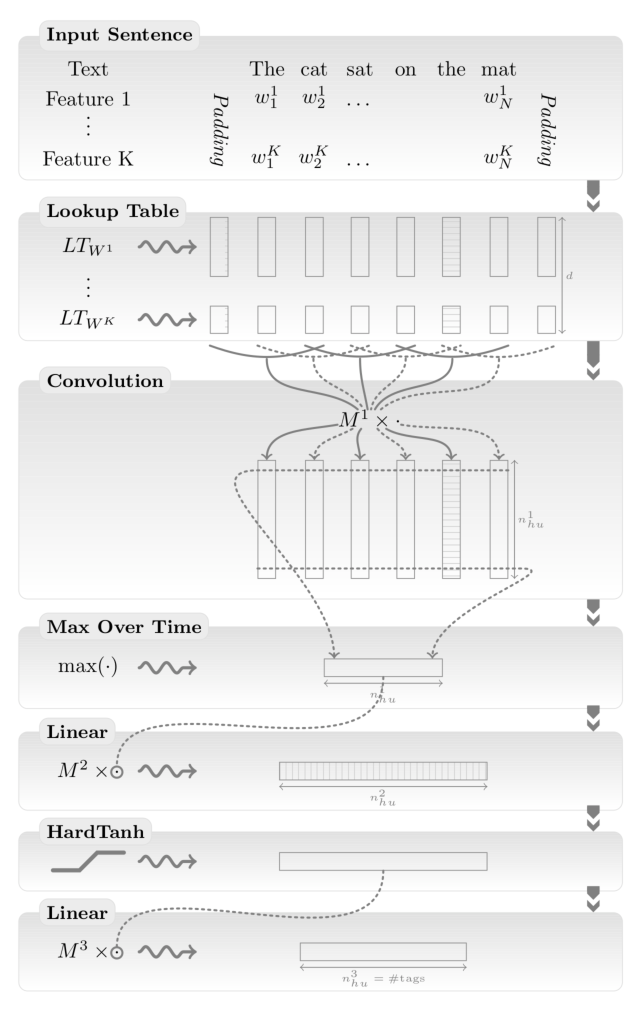
\includegraphics[width=\textwidth]{ch03-collobert-sentence2011}
          \caption{Neural network with a sentence approach.}
          \label{fig:collobert-sentence2011}
        \end{subfigure}
        \caption[Window and sentence approach networks used
        by~\citeauthor{collobert2011natural}]{Neural network architectures used
        by~\citep{collobert2011natural}. The lookup tables contain the word
        embeddings, which are then used to compute an output vector representing
        the predictions of the network for a given NLP task.}
        \label{ch03:fig:collobert2011}
      \end{figure}

    \subsubsection{Word2vec}
      The architectures proposed by~\citeauthor{collobert2011natural}
      \citep{collobert2008unified, collobert2011natural} allow one to learn word
      embeddings but they still need some labeled data for training. Labels are
      not used to help the model to know what the values of the embeddings
      should be but to help the model to learn representations which contain
      information that is useful to predict the correct output and solve a given
      NLP task. Therefore, this semi-supervised learning still requires some
      human labor to annotate examples and get labels.
      \citeauthor{mikolov2013efficient}~\citep{mikolov2013efficient} proposed
      the novel \texttt{word2vec} model to overcome this problem. Instead of
      using NLP tasks as a proxy to know which information should be encoded
      into word embeddings,~\citeauthor{mikolov2013efficient} learn the
      distribution of embeddings across the vectorial space $\mathbb{R}^d$ with
      the hypothesis of John Rupert Firth~\citep{firth1961papers}: \textit{``You
      should know a word by the company it keeps.''}. Their model considers that
      the vectors of the words in a window should be enough to predict what are
      the other words in the window. Let ($w_{t-n}, ~\dots, ~w_{t-1}, ~w_t,
      ~w_{t+1}, ~\dots, ~w_{t+n}$) be a sequence of words composed of a central
      word $w_t$ and the $2n$ words around it. This sequence of words is called
      \textit{a window}. The authors actually propose two different
      architectures of their model:

      \begin{itemize}
        \item Continous Bag-of-Words (CBOW): in this architecture, the goal is
          to predict the central word $w_t$ given all the other words of the
          window. This is represented in the left part
          of~\autoref{ch03:fig:cbow-skipgram}.
        \item Skip-gram: in this architecture, the goal is to predict all the
          words of the sequence except the central word $w_t$, which is used as
          the input. This is represented in the right part
          of~\autoref{ch03:fig:cbow-skipgram}.
      \end{itemize}

      \begin{figure}[h!]
        \centering
        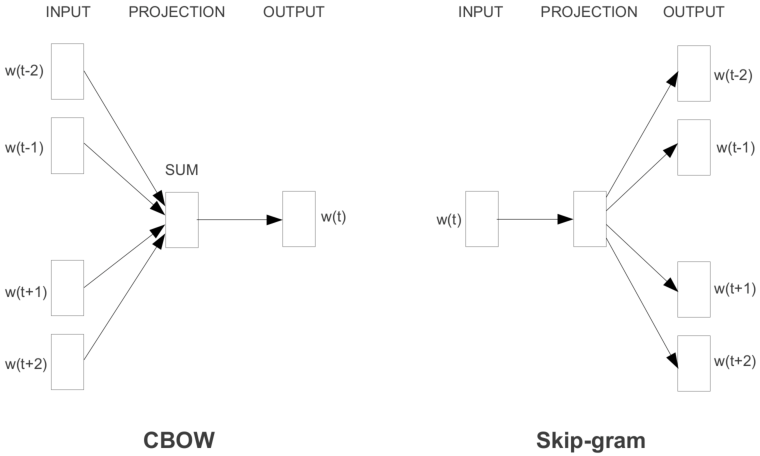
\includegraphics[width=0.87\textwidth]{ch03-cbow-skipgram-architecture}
        \caption[CBOW and Skip-gram model used
        by~\citeauthor{mikolov2013efficient}]{Continuous Bag-of-Words (CBOW) and
        Skip-gram models, respectively on left and right part of the image, used
        in~\citep{mikolov2013efficient}}
        \label{ch03:fig:cbow-skipgram}
      \end{figure}

      \noindent Both architectures are trained to maximize the probability of
      predicting the correct words (in fact, they maximize the $log$ probability
      because it simplifies the computations of the derivatives for a gradient
      descent training). Their objective is therefore slightly different:

      \begin{itemize}
        \item in CBOW, the objective is to maximize the probability of
          predicting the central word $w_t$ given the context sequence,
          \textit{i.e.} to maximize:
          \begin{equation}
            \log\big(P(w_t~|~w_{t-n},~\dots,~w_{t-1},~w_{t+1},~\dots,~w_{t+n})\big) =
            \log\big(P(w_t~|~\theta)\big)
          \end{equation}
          where $\theta$ is the average vector of the vectors of words in
          ($w_{t-n}, ~\dots, ~w_{t-1}, ~w_{t+1}, ~\dots,$ $~w_{t+n}$). With the
          embedding vector of the word $w_j$ noted as $\mathbf{v}_j$, it is
          defined as:
          \begin{equation}
            \theta = \frac{1}{2n}
                     ~\sum_{\substack{-n \leq j \leq n \\ j \neq 0}}
                     \mathbf{v}_{t+j}
          \end{equation}
        \item in Skip-gram, the objective is to maximize the probability of
          predicting each one of the different words of the context given the
          central word $w_t$, \textit{i.e.} to maximize:
          \begin{equation}
            \sum_{\substack{-n \leq j \leq n \\ j \neq 0}}
            \log\big(P(w_{t+j}~|~w_t)\big)
          \end{equation}
      \end{itemize}

      In both models, the probability of predicting a word is computed with the
      embeddings of the words involved. In~\citep{mikolov2013efficient}, there
      are two embedding matrices (\textbf{WI} and \textbf{WO}, respectively for
      \textit{Input} and \textit{Output}) which both contain the embedding of
      each word of a vocabulary so all words are actually represented with two
      different vectors (one from \textbf{WI} and another one from \textbf{WO}).
      When a word is used as the input of the neural network (in CBOW, input
      words are the context words; in Skip-gram it is the central word), the
      corresponding word embedding is selected from the \textbf{WI} matrix. When
      a word is used as the output of the neural network (in CBOW, the output
      word is the central word; in Skip-gram they are the context words), word
      embeddings from the \textbf{WO} matrix are selected. The probability of
      predicting a word given another word is expressed with the softmax
      function and is defined as:

      \begin{equation}
        P(w_i~|~w_j) = \frac{\exp(\mathbf{v'}_{i} {}^\top~ \mathbf{v}_{j})}
              {\sum_{w \in \mathcal{V}} \exp(\mathbf{v'}_{w} {}^\top~ \mathbf{v}_{j})}
      \end{equation}
      where $\mathbf{v}$ (resp. $\mathbf{v'}$) refers to embeddings selected in
      the \textbf{WI} (resp. \textbf{WO}) matrix, and $\mathcal{V}$ is the
      vocabulary containing all words. Computing the softmax function is
      computationally expensive because it needs to iterate over all the words
      in the vocabulary $\mathcal{V}$, which can contain millions of words.
      \citeauthor{mikolov2013efficient} \citep{mikolov2013efficient} introduced
      the negative sampling to simplify this expression, which is based on the
      noise-contrastive estimation~\citep{gutmann2012noise, mnih2012fast}. The
      idea is to randomly select only a fraction of words from the vocabulary
      and constrain the model to predict the expected correct word with a higher
      probability than for those randomly selected words. The probability of
      predicting a word becomes:

      \begin{equation}
        \log\big(P(w_i~|~w_j)\big) =
        \log \big( \sigma(\mathbf{v'}_{i} {}^\top~\mathbf{v}_{j}) \big)
              + \sum_{l=1}^k \mathbb{E}_{w_l \sim P_k(w_j)}
                \log \big( \sigma(\mathbf{-v'}_{l} {}^\top~\mathbf{v}_{j}) \big)
      \end{equation}
      where $\sigma$ is the sigmoid function defined as $\sigma(x) = \frac{1}{1
      + e^{\text{-}x}}$ and $P_k(w_j)$ is a random noisy distribution created by
      selecting $k$ random words different from $w_j$ from the vocabulary
      $\mathcal{V}$. The final objective function of CBOW and Skip-gram models
      is obtained by maximizing the log probability over all the possible
      context/central word pairs of windows of size $n$ across a corpus of size
      $T$. For Skip-gram, the objective of the model is to maximize:

      \begin{equation}
        \label{ch03:eq:sgns}
        \begin{split}
          & \frac{1}{T} \sum_{t=1}^T
          \sum_{\substack{-n \leq j \leq n \\ j \neq 0}}
          \log\big(P(w_{t+j} | w_t)\big) \\
        = & \frac{1}{T} \sum_{t=1}^T
          \sum_{\substack{-n \leq j \leq n \\ j \neq 0}}
          \Big(
            \log \big( \sigma(\mathbf{v'}_{t+j} {}^\top~\mathbf{v}_{t}) \big)
            + \sum_{i=1}^k \mathbb{E}_{w_i \sim P_k(w_t)}
            \log \big( \sigma(\mathbf{-v'}_{i} {}^\top~\mathbf{v}_{t}) \big)
          \Big)
        \end{split}
      \end{equation}
      Models are trained by iterating through the corpus several times (each
      full iteration is called an \textit{epoch}). After a certain number of
      epoch are done, final word embedding for each word of the vocabulary is
      obtained by averaging its two embeddings from \textbf{WI} and \textbf{WO}.
      \medskip

      CBOW and Skip-gram models are unsupervised machine learning models. They
      do not use any labels during training but only consider cooccurrences of
      words inside windows to learn the values of word embeddings. However, they
      are able to encode linguistic information.~\citet{mikolov2013efficient}
      show that embeddings learned by their \texttt{word2vec} model perform well
      in the word analogy task ($0.53$ for Skip-gram vs. $0.11$ for the neural
      network model of \citep{collobert2008unified}) as well as in a sentence
      completion challenge ($0.64$ for CBOW vs. $0.51$ for the model of
      \citep{bengio2003neural}).
      \citeauthor{arora2015random}~\citep{arora2015random} have proposed to
      explain the reasons of the existence of linear relations in word
      embeddings. Starting with a generative model, they perform a random walk
      on word vectors instead of sequentially looking at the word windows of a
      large corpus. They compute the probability that two words appear in the
      same window with the random walk and demonstrate theoretically the
      emergence of relationships between words and why one can find linear
      relationships in word embeddings learned with the \texttt{word2vec} model.

    \subsubsection{Fasttext}
      While word embeddings learned by the CBOW or the Skip-gram objective
      functions are able to capture semantic properties of words like the
      feminine attribute of the word ``queen'' compared to the word ``king'',
      they are lacking some syntactic properties. Indeed, in those models, words
      are considered as global independent entities but in languages like
      English, words that share common letters or subgroups of letters are often
      related.  For example, in English, adverbs typically end with the suffix
      \textit{-ly}.  Similarly, prefixes can also indicate that words are
      related like for the words ``possible'' and ``impossible'', and common
      etymological roots also tell information about similar words like for the
      words ``telephone'' and ``microphone''.  This observation is at the origin
      of the idea developed
      by~\citeauthor{bojanowski2016enriching}~\citep{bojanowski2016enriching}.
      Instead of considering a word as a single entity, they consider it as a
      set of \textit{n-grams}, \textit{i.e.} groups of subwords with length
      between 2 and 6 letters. For example, the word ``badly'' is decomposed as:
      \{``ba'', ``ad'', ``dl'', ``ly'', ``bad'', ``adl'', ``dly'', ``badl'',
      ``adly'', ``badly''\}. This information is plugged into a
      \texttt{word2vec} Skip-gram model to produce a novel model called
      \texttt{fasttext} where words are replaced by combination of n-grams. Each
      n-gram is associated to its own vectors in the embedding matrices
      \textbf{WI} and \textbf{WO}, so the model learns simultaneously embeddings
      of words and embeddings of n-grams. After training, only word embeddings
      are kept for future use but embeddings of n-grams help the model to
      understand the morphological similarities between words. \medskip

      When the \texttt{fasttext} model is evaluated on the word analogy task,
      results are greatly improved especially on the syntactic evaluation
      dataset because embeddings are able to capture linguistic information to
      learn that ``great'' and ``greatly'' have the same relation as ``bad'' and
      ``badly''. Moreover, the \texttt{fasttext} model presents other great
      advantages. First, in CBOW and Skip-gram models, words that are not in the
      training corpus are not seen and therefore do not have a learned word
      embedding associated to them. With \texttt{fasttext}, it is possible to
      construct a word embedding for such words (called
      \textit{out-of-vocabulary} words) because the vector of a word can be seen
      as the sum of the vectors of its n-grams. The n-grams solution proposed
      by~\citeauthor{bojanowski2016enriching}~\citep{bojanowski2016enriching}
      allows one to create embeddings for new unseen words without having to
      re-train the model on a new corpus containing those new words. Second,
      words occuring rarely in a text are less frequently seen in approaches
      which iterate through the corpus with a sliding window of words like in
      \texttt{word2vec} or in \texttt{fasttext}. Therefore, representations of
      rare words is often not as good as the representations of frequent words.
      However, \texttt{fasttext} also learns a representation for n-grams. A
      rare word like ``interconnectedness'' which shares common n-grams with the
      words ``connect'' or ``connection'' can still capture semantic information
      in its embedding because the words ``connect'' or ``connection'' are more
      frequently seen in different contexts and the representations of their
      n-grams are more frequently updated to encode this information.
      \texttt{fasttext} is therefore better than \texttt{word2vec} to learn the
      representations of rare words because of the use of n-grams in the model
      (on a word semantic similarity task, word embeddings learned by
      \texttt{fasttext} obtain a score of $0.47$ on the Rare-Words
      dataset~\citep{luong2013better} while vectors learned by the
      \texttt{word2vec} Skip-gram and CBOW models obtain $0.43$).

  \subsection{Matrix factorization}
    \label{ch03:subsec:matrix-factorization}
    The methods presented in the previous subsection rely on a neural network
    architecture and a sliding window approach to learn word embeddings. These
    methods use the cooccurrence information between words to train the vectors
    of words such that words cooccurring frequently together in context windows
    have similar word vectors. However, the information they use to learn word
    embeddings is only local information (context windows). Matrix factorization
    methods use different statistical information of the training corpus by
    considering the global cooccurrence count of words instead of their local
    ones as in context windows. Since the vocabulary of the corpus can be in the
    order of millions, using the global word cooccurrences matrix as the
    embedding matrix is not feasible, so these approaches factorize the global
    cooccurrence information matrix with singular value decomposition (SVD) and
    truncate it to keep only the first $k$ dimensions in order to obtain a
    smaller matrix with approximated properties, which is used as the embedding
    matrix. \medskip

    One of the first work in global matrix factorization is \textit{Latent
    Semantic Analysis} (LSA) \citep{deerwester1990lsa} which uses a matrix
    containing the number of occurrences of words in several documents. Another
    similar method~\citep{lund1996hal} factorizes a matrix containing the
    information about the cooccurrence of words in context windows. A
    formalization of a more general matrix factorization approach has been
    described in~\citep{turney2012domain, levy2014factorization}. Let
    $\widetilde{\mathbf{M}}$ be a matrix containing cooccurrence information of
    words obtained from a text corpus and let $\widetilde{\mathbf{M}} =
    \mathbf{U} \mathbf{D} \mathbf{V}^\top$ be its singular value decomposition.
    A word embedding matrix $\mathbf{M}$ containing $k$-dimensional word vectors
    is obtained with:

    \begin{equation}
      \mathbf{M} = \mathbf{U}_{1:k} \mathbf{D}_{1:k, 1:k}^\alpha
    \end{equation}
    where $\mathbf{U}_{1:k}$ is the matrix $\mathbf{U}$ truncated to keep only
    the first $k$ columns, $\mathbf{D}_{1:k,1:k}$ is the matrix $\mathbf{D}$
    truncated to keep only the first $k$ rows and $k$ columns and $\alpha \in
    [0,1]$. \medskip

    Another common method used to learn word embeddings is
    \texttt{GloVe}~\citep{pennington2014glove}. While \texttt{GloVe} is not
    based on SVD like the other methods, it has been shown that the objective
    function of \texttt{GloVe} is an implicit factorization of the logarithm of
    the global word cooccurrence count matrix~\citep{levy2015improving}. For
    each possible pair of words $(w_i, w_j)$ with $w_i, w_j \in \mathcal{V}$
    (where $\mathcal{V}$ is the vocabulary of the text corpus), the
    \texttt{GloVe} model aims to learn word vectors such that:

    \begin{equation}
      \mathbf{v}_i^\top ~\mathbf{v}_j + b_i + b_j =
        \log(1 + \widetilde{\mathbf{M}_{ij}})
    \end{equation}
    where $\mathbf{v}_i$ (resp. $\mathbf{v}_j$) is the word vector of the word
    $w_i$ (resp. $w_j$), $b_i$ and $b_j$ are some bias related to the words
    $w_i$ and $w_j$ and $\widetilde{\mathbf{M}_{ij}}$ is the number of times the
    word $w_i$ occurs in the context of the word $w_j$. The vector of each word
    of the vocabulary $\mathcal{V}$ is obtained by training the model to
    minimize the global loss function $J$, defined as:

    \begin{equation}
      J = \sum_{i, j=1}^{|\mathcal{V}|}
        \lambda_{ij}
        \big(\mathbf{v}_i^\top ~\mathbf{v}_j + b_i + b_j -
             \log(1 + \widetilde{\mathbf{M}_{ij}})
        \big)^2
    \end{equation}
    where $\lambda_{ij}$ is a weight depending on the value of
    $\widetilde{\mathbf{M}_{ij}}$ so that pairs of words with a zero or a small
    cooccurrence count do not have a lot of importance in the loss function.
    \pagebreak

\section{Improving word embeddings with external resources}
  \label{ch03:sec:external-resources}
  General methods to learn word embeddings, whether by using a neural network
  approach (presented in~\autoref{ch03:subsec:neural-network}) or a matrix
  factorization approach (presented
  in~\autoref{ch03:subsec:matrix-factorization}) mainly use training text
  corpora like Wikipedia articles or crawled content from the Web. While those
  corpora contain a lot of information, their content is rather generic, in a
  sense that specific information about words is not present. Semantic relations
  like synonymy, antonymy, hypernymy, etc. are not explicitly written in those
  corpora and it is unlikely that two words linked with such relations cooccur
  within the same window or at least not often enough together for the model to
  encode this kind of relation between words into their embeddings. To overcome
  this problem, several methods have been proposed to improve the linguistic
  information contained in word embeddings with other additional sources of
  knowledge. Approaches to improve word embeddings with other sources of
  knowledge can be separated into two main categories: either by using
  additional knowledge during training or either by using it after training.
  \medskip

  The first category uses additional knowledge \textbf{during the training} of
  word embeddings.
  \citeauthor{yudredze2014improving}~\citep{yudredze2014improving} extract
  synonym information from WordNet~\citep{miller1995wordnet} and a paraphrase
  database (PPDB)~\citep{ganitkevitch2013ppdb}. This new information is used in
  a \texttt{word2vec} CBOW model to add new constraints between some related
  words. Embeddings learned with this method have better results on a word
  semantic similarity task, demonstrating that using additional information
  during training can improve word embeddings.
  \citeauthor{kiela2015specializing}~\citep{kiela2015specializing} improve both
  the similarity and the relatedness information encoded into word embeddings by
  using respectively synoyms and word associations into a \texttt{word2vec}
  Skip-gram model. Embeddings are then evaluated on a word semantic similarity
  and a synonym detection tasks where the results are improved in both tasks
  compared to a regular Skip-gram model. \medskip

  The second category uses additional knowledge \textbf{after the word
  embeddings have been learned}, as a post-training step.
  \citeauthor{faruqui2015retrofitting}~\citep{faruqui2015retrofitting} propose
  to extract pairs of related words from semantic lexicons resources like
  WordNet~\citep{miller1995wordnet}, Framenet~\citep{baker1998berkeley} or
  PPDB~\citep{ganitkevitch2013ppdb}. Pairs are used to update the
  representations and move closer the embeddings of words in those pairs, in a
  method called \texttt{retrofitting}. Like the other methods that use
  additional knowledge during training, embeddings learned with
  \texttt{retrofitting} give better performances in tasks like word semantic
  similarity, synonym detection or sentiment analysis. The \texttt{retrofitting}
  method was extended by~\citet{jo2018extrofitting} in a novel method called
  \texttt{extrofitting}. In addition to updating word embeddings values with
  extracted pairs, the authors change the number of dimensions in vectors before
  doing any modifications and they reorganize the vectors based on the
  additional knowledge so both word embeddings and the vector space benefit from
  the additional information found in semantic lexicons. Final
  \texttt{extrofitting} word embeddings perform better than
  the~\citeauthor{faruqui2015retrofitting} retrofitted vectors on a word
  semantic similarity task ($+3.46\%$ on average on the MEN
  dataset~\citep{bruni2014multimodal} when improving \texttt{GloVe} embeddings
  of various sizes) which were already better than original vectors learned by
  the \texttt{GloVe} model.

\section{Contextual word representations}
  In all the methods presented so far for learning word embeddings, whether by
  using directly large text corpora like in \texttt{word2vec}, \texttt{fasttext}
  or \texttt{GloVe} or by using additional external information like in
  \texttt{retrofitting}, each word of the vocabulary is associated to a single
  word vector. However, some words in a language are \textit{polysemous}: their
  meaning can be different depending on the context in which they are used. In
  the two following sentences, the word ``mouse'' has different meanings:
  \begin{enumerate}
    \item The \textit{mouse} is chased by the cat.
    \item I am using the \textit{mouse} to move the cursor on my screen.
  \end{enumerate}

  \noindent In the first sentence, the word ``mouse'' refers to the small
  animal. In the second sentence, it refers to the peripheral device plugged
  into a computer to perform some actions. If a single unique vector is
  associated to the word ``mouse'', should this vector be close to the vectors
  of other animals or close to the vectors of the words ``screen'' and
  ``keyboard''? There are no optimal solutions in this case but rather a clear
  evidence of the shortcoming of methods that associate the same vector to all
  the occurrences of a polysemous word: they cannot properly encode that words
  can have multiple meanings and thus different vector representations.

  \subsection{Sense embeddings}
    \citeauthor{neelakantan2014efficient}~\citep{neelakantan2014efficient}
    propose to solve this shortcoming by learning a different vector for each
    sense of a word. Each word $w$ of a vocabulary $\mathcal{V}$ is assigned to:
    \begin{itemize}
      \item a global vector $\mathbf{v_g}(w)$;
      \item a sense vector $\mathbf{v_{s, k}}(w)$ for each one of its senses,
        where $k \in [1,~\dots,~K_w]$ and $K_w$ is the number of senses of the
        word $w$.
    \end{itemize}

    \noindent They use the \texttt{word2vec} Skip-gram model of
    \cite{mikolov2013distributed} to learn sense vectors and global vectors. For
    each central word $w_t$ of a sequence of words and its associated context
    window $c_t = (w_{t-n}, ~\dots, ~w_{t-1}, ~w_{t+1}, ~\dots, ~w_{t+n})$, they
    compute the context vector of this window by averaging the global vectors of
    each word $c$ in the context $c_t$:

    \begin{equation}
      \mathbf{v_{context}}(c_t) = \frac{1}{2n} \sum_{c \in c_t} \mathbf{v_g}(c)
    \end{equation}
    They determine which sense $s_t$ of $w_t$ is used in this context $c_t$ by
    finding the closest sense vector $\mathbf{v_{s, k}}(w_t)$ to the context
    vector $\mathbf{v_{context}}(c_t)$:

    \begin{equation}
      s_t = \argmax_{k \in [1,~\dots,~K_{w_t}]}
            ~sim(\mathbf{v_{s, k}}(w_t), \mathbf{v_{context}}(c_t))
    \end{equation}
    where $sim()$ is a similarity function between two vectors like the cosine
    similarity function. After finding the sense $s_t$ of $w_t$ closest to the
    context $c_t$, they use the Skip-gram objective function and the gradient
    descent technique to update the values of the sense vector $\mathbf{v_{s,
    s_t}}$ of the word $w_t$ and the values of the context vector
    $\mathbf{v_{context}}(c_t)$ by maximizing:

    \begin{equation}
      \log\big(P(\mathbf{v_{s, s_t}}(w_t)~|~\mathbf{v_{context}}(c_t))\big)
    \end{equation}
    This approach has the advantage of not needing human labeling on data,
    because the sense $s_t$ of the word $w_t$ used in the context $c_t$ is found
    on its own by the method. Other approaches
    like~\citep{iacobacci2015sensembed} use a word sense disambiguation tool to
    automatically add a suffix to words with different senses. With the small
    previous example above, it would annotate the word ``mouse'' like
    ``$mouse_1$'' and ``$mouse_2$''. The \texttt{word2vec} CBOW
    model~\citep{mikolov2013efficient} is then applied on the disambiguated
    corpus to learn one vector per sense. This approach has the inconvenient of
    needing a tool to disambiguate the corpus which is often based on a manually
    generated external source of knowledge.

  \subsection{Contextualized word embeddings}
    As said in the previous subsection, words can have different meanings
    depending on the context in which they are used. While some approaches learn
    to associate a vector to each sense of each
    word~\citep{neelakantan2014efficient, iacobacci2015sensembed}, they neglect
    the information one can found inside words, like in \texttt{fasttext}
    ~\citep{bojanowski2016enriching}which uses subword information to learn
    morphological properties of words. Moreover, knowing which sense of a word
    is used in a context can require an external disambiguation tool. Another
    recent way to tackle the issue of learning representations for polysemous
    words is to shift from word representations to occurrence representations.
    That is, instead of associating one embedding per word or per word sense
    (learned based on all the contexts in which they occur in a corpus), it
    could be interesting to have one context-specific embedding for each
    occurrence of a word in a corpus. This would relax the constraint of
    optimizing the representations for all the occurrences of a word (or its
    senses) while providing a very fine-tuned representation of a word in a
    given context. Those types of approaches are called \textit{contextualized
    word embeddings}~\citep{peters2018elmo, devlin2019bert, liu2019roberta} and
    have been proven to be very popular within the last couple of years. In what
    follows, we present the main approaches that fall into this category.
    \medskip

    \citeauthor{peters2018elmo}~\citep{peters2018elmo} propose a novel
    architecture to learn a \textit{contextual representation} of words without
    requiring any labeled data or external tools for disambiguation. Their
    architecture is based on bidirectional LSTM~\citep{huang2015bidirectional}
    and is represented in~\autoref{ch03:fig:elmo-model}. Their model is called
    \texttt{ELMo} for \textbf{E}mbeddings from \textbf{L}anguage
    \textbf{Mo}dels. It relies on the objective function of a language model. As
    a reminder, in a language model the objective is to be able to successively
    predict words in a sentence given all the previous words of this sentence.
    For example, with the sentence ``The mouse is chased by the cat.'', the
    model aims to predict the word ``chased'' given the words ``The'', ``mouse''
    and ``is''. More formally, it is equivalent to maximize:

    \begin{equation}
      P(t_1, ~t_2, ~\dots, ~t_n) = \prod_{k=1}^n P(t_k~|~t_1,~\dots,~t_{k-1})
    \end{equation}

    \begin{figure}[b!]
      \centering
      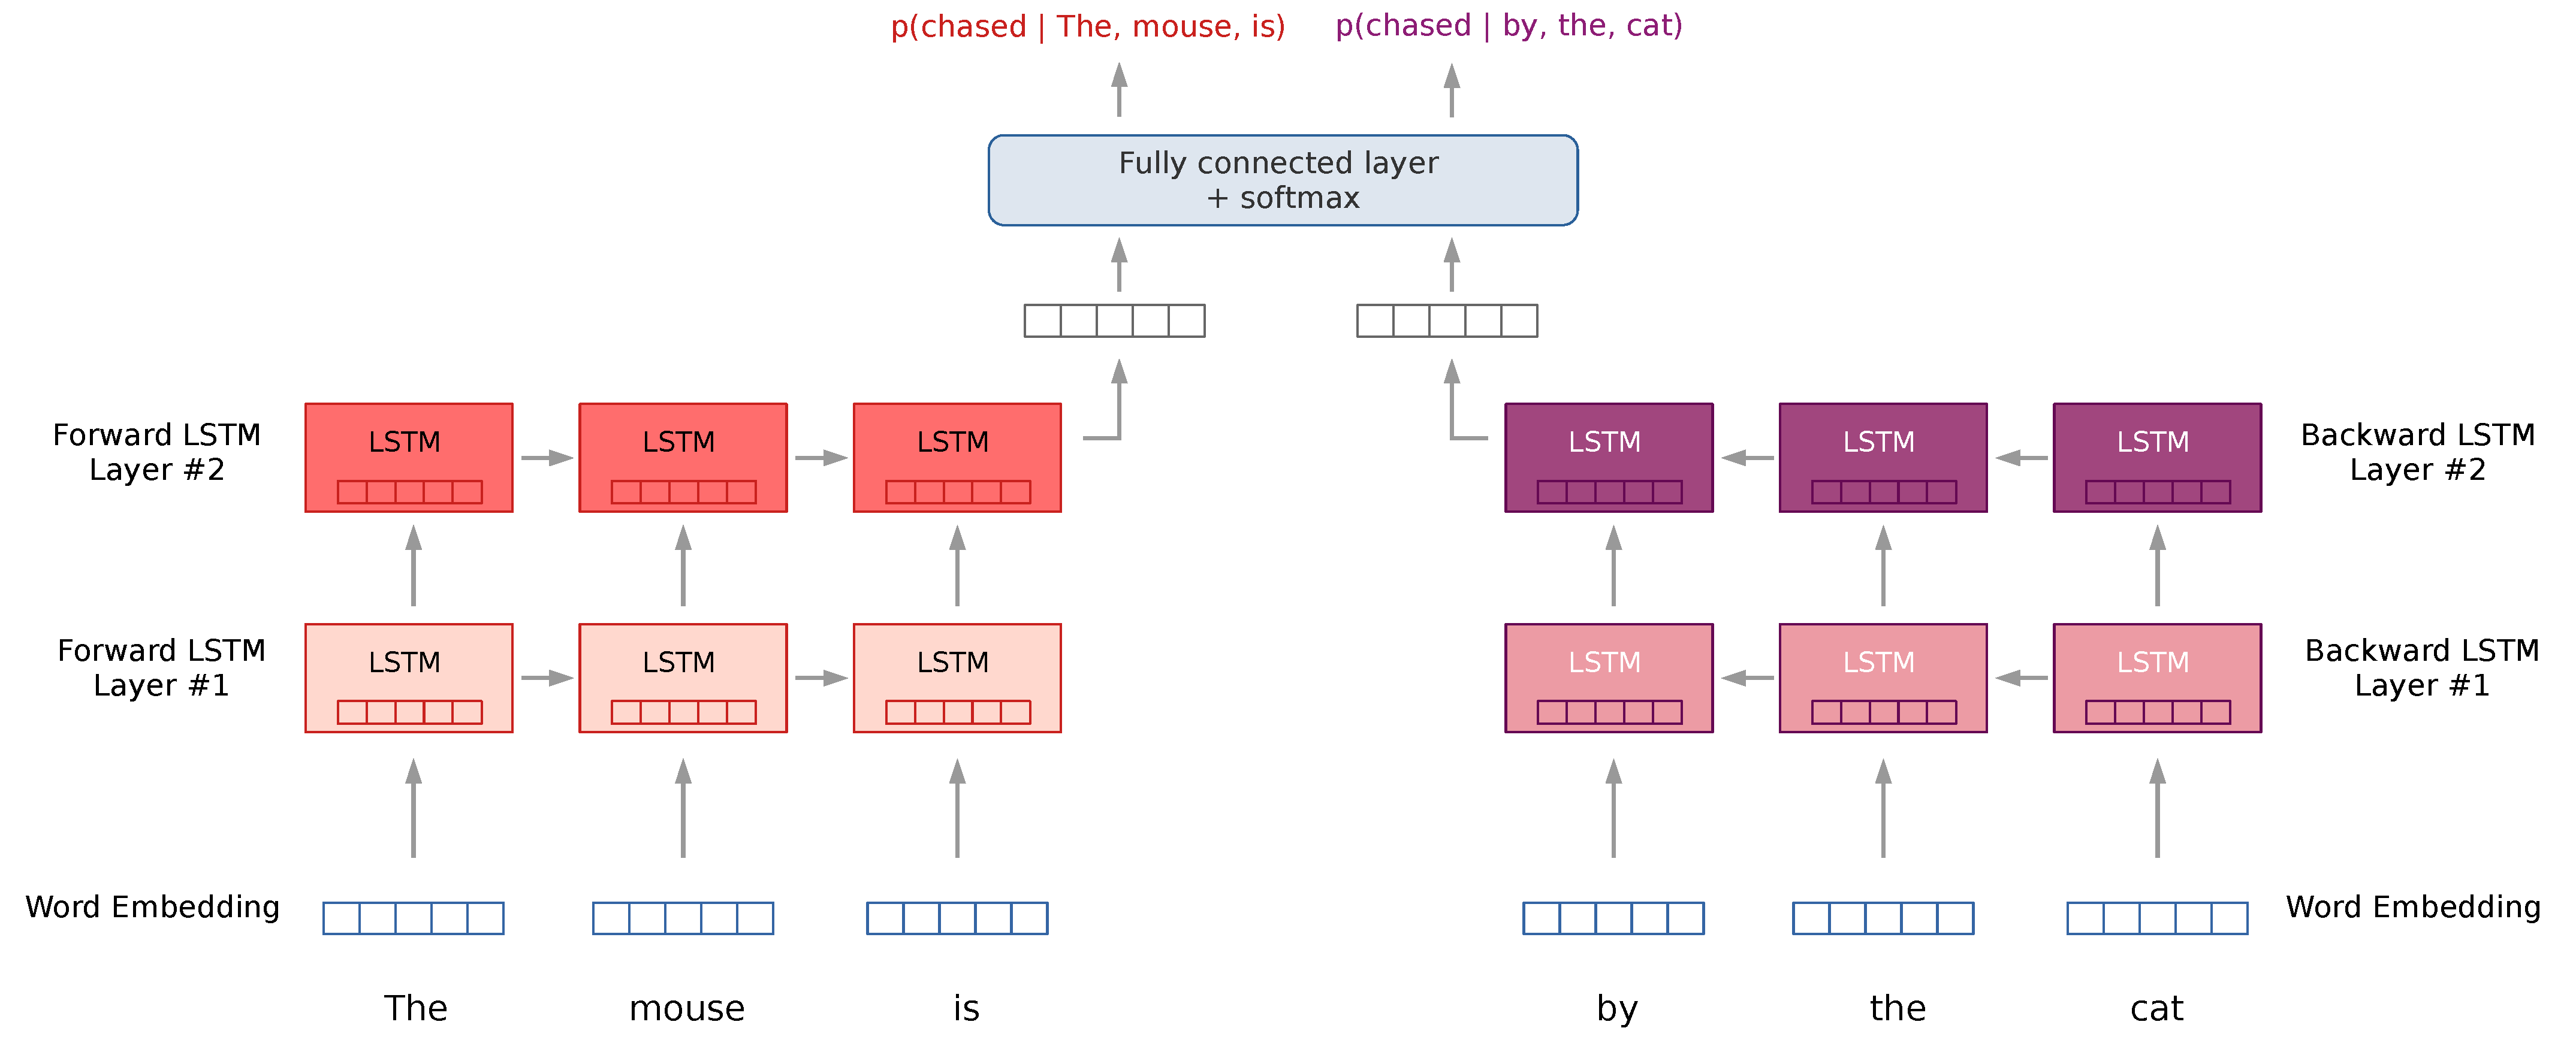
\includegraphics[width=\textwidth]{ch03-elmo-architecture}
      \caption[Architecture of the \texttt{ELMo} model from
      \citeauthor{peters2018elmo}.] {Architecture of the \texttt{ELMo} model
      from~\citep{peters2018elmo}. It is composed of 2 bidirectional LSTM layers
      (bi-LSTM). Each word is associated to its own word embedding which is
      used as the input in the first bi-LSTM layer. The outputs of the first
      bi-LSTM layer are then passed to the second bi-LSTM layer. The final
      representation of a word in a context is a combination of its own word
      embedding and the outputs of both bi-LSTM.}
      \label{ch03:fig:elmo-model}
    \end{figure}

    \medbreak
    \noindent \texttt{ELMo} also models the language in the backward direction,
    \textit{i.e.} to predict a word given all the words that come after it. This
    is equivalent to maximize:

    \begin{equation}
      P(t_1,~t_2,~\dots,~t_n) = \prod_{k=1}^n P(t_k~|~t_{k+1},~\dots,~t_{n})
    \end{equation}
    The objective of the \texttt{ELMo} model is to maximize the log likelihood
    of predicting words in both directions, \textit{i.e.} to maximize:

    \begin{equation}
      \begin{split}
      \log P(t_1,~t_2,~\dots,~t_n) = \sum_{k=1}^n
        \Big(
      & \log \big(P(t_k~|~t_1,~\dots,~t_{k-1};
             \overrightarrow{\Theta}_{LSTM},\Theta)\big)~+\\
      & \log \big(P(t_k~|~t_{k+1},~\dots,~t_{n};
             \overleftarrow{\Theta}_{LSTM},\Theta)\big)
        \Big)
      \end{split}
    \end{equation}
    where $\overrightarrow{\Theta}_{LSTM}$ (resp.
    $\overleftarrow{\Theta}_{LSTM}$) are the parameters of the forward (resp.
    backward) bi-LSTM layers and $\Theta$ are the shared parameters between the
    bi-LSTM (the embeddings of words and the weights of the fully connected and
    the softmax layers). \medskip

    Bidirectional LSTM (bi-LSTM) compute an internal representation for each
    word position $k$ in each layer $j$. For forward LSTM (red boxes
    in~\autoref{ch03:fig:elmo-model}), each internal representation is noted as
    $\overrightarrow{\mathbf{h}}_{k, j}^{LM}$. For backward LSTM (purple boxes
    in~\autoref{ch03:fig:elmo-model}), each internal representation is noted as
    $\overleftarrow{\mathbf{h}}_{k, j}^{LM}$. As an example,
    $\overrightarrow{\mathbf{h}}_{3, 2}^{LM}$ is the internal representation of
    the right dark red box in~\autoref{ch03:fig:elmo-model}, while
    $\overleftarrow{\mathbf{h}}_{2, 1}^{LM}$ is the internal representation of
    the middle light purple box in~\autoref{ch03:fig:elmo-model}. After the
    objective function of \texttt{ELMo} has been trained to be maximized over a
    large text corpus, \texttt{ELMo} is able to compute a unique representation
    for each word based on their context. To compute the contextual
    representation of the word $w_t$ from the context $c_t = (w_1,
    ~\dots,~w_{t-1},~w_{t+1},~\dots,~w_{t+n})$, \texttt{ELMo} computes the
    internal representations of bi-LSTM layers with the embedding of each word
    in the context $c_t$ and then sums the internal representations, that is:

    \begin{equation}
      \label{ch03:eq:elmo-vector}
      \mathtt{ELMo}(w_t) = \sum_{j = 0}^N \mathbf{h}_{t, j}^{LM}
    \end{equation}
    where $\mathbf{h}_{t, j}^{LM}$ is the concatenation of the forward and
    backward representations of the word $w_t$ in the $j$-th bi-LSTM layer
    (\textit{i.e.} $\mathbf{h}_{t, j}^{LM} = [\overrightarrow{\mathbf{h}}_{t,
    j}^{LM},~~ \overleftarrow{\mathbf{h}}_{t, j}^{LM}]$). For $j = 0$, the word
    embedding of the word $w_t$ is concatenated with itself (\textit{i.e.}
    $\mathbf{h}_{t, 0}^{LM} = [\mathbf{x}_t^{LM}, \mathbf{x}_t^{LM}]$). In the
    \texttt{ELMo} model, there are only 2 bi-LSTM layers (so $N = 2$
    in~\autoref{ch03:eq:elmo-vector}). \medskip

    The approach of \texttt{ELMo} to learn contextualized word representations
    has led to many other methods which have been proven to bring large increase
    of performances in downstream NLP tasks~\citep{devlin2019bert,
    liu2019roberta}. In~\citeyear{devlin2019bert},
    \citeauthor{devlin2019bert}~\citep{devlin2019bert} proposed an architecture
    deeper than \texttt{ELMo} to model context information into word
    representations. Their model is called \texttt{BERT} (for
    \textbf{B}idirectional \textbf{E}ncoder \textbf{R}epresentations from
    \textbf{T}ransformers) and is composed of 12 layers (24 in the larger
    version of \texttt{BERT}, only 2 in the \texttt{ELMo} model). Each layer is
    a bidirectional transformer~\citep{vaswani2017attention} which uses context
    information from before and after a token to compute its word
    representation. During training, \texttt{BERT} randomly masks 15\% of the
    words in sentences (by replacing them with a \texttt{[MASK]} token or with a
    random word) and tries to predict the original non-masked words given their
    context instead of predicting the next word of a sequence given all the
    previous words of this sequence like in a classic language model.
    \texttt{BERT} has recently been integrated into the Google search engine and
    has been considered by Jeff Dean as one of the biggest advances in the
    development of this search engine. \medskip

    Given the large increase of performances in multiple downstream tasks with
    the representations learned by \texttt{BERT}, many works have extended this
    architecture (and also the name of the model): to optimize the training time
    (\texttt{ALBERT}~\citep{lan2019albert}), to train on larger corpora with
    more layers (\texttt{RoBERTa}~\citep{liu2019roberta}), to specialize on
    another language like French (\texttt{FlauBERT}~\citep{le2019flaubert},
    \texttt{CamemBERT}~\citep{martin2019camembert}), etc.

\section{Overview and recap}
  \label{ch03:sec:overview-methods}
  In the previous subsections, we have described common methods used to learn
  word representations. Presented methods can be very diverse: using only
  cooccurrences of words inside a sliding window, using additional external
  knowledge or using context information of words. In this subsection, we are
  going to present an overview of all the methods presented so far and how they
  compare to each other with their strenghts and weaknesses.

  \subsection{Visualization of methods to learn word embeddings}
    A simple (and subjective) way to visually classify the different methods to
    learn word embeddings is to compare them on two criteria:

    \begin{enumerate}
      \item Does the method use a large architecture to learn word embeddings?
      \item How much linguistic information is used during the learning of word
        embeddings?
    \end{enumerate}

    \noindent \autoref{ch03:fig:overview-methods} represents the methods
    described in this chapter along two axes:

    \begin{itemize}
      \item The horizontal axis represents the relative size of the architecture
        used in different methods. Methods that use small architectures (like a
        single hidden layer neural network in~\citep{collobert2008unified}) are
        placed on the left of this axis. Models with larger architectures like
        \texttt{ELMo}~\citep{peters2018elmo} or
        \texttt{BERT}~\citep{devlin2019bert} are placed on the right of this
        axis.
      \item The vertical axis indicates (on a relative scale, not an absolute
        one) how much linguistic information is used during training to learn
        word embeddings. The more information a model uses (like external
        knowledge or context information in addition to solely using a text
        corpus), the higher it is placed on this axis.
    \end{itemize}

    A clear trend can be observed in~\autoref{ch03:fig:overview-methods}: the
    more linguistic information a model uses, the larger it is.
    \citeauthor{collobert2011natural}~\citep{collobert2011natural} extend the
    model of \citeauthor{collobert2008unified}~\citep{collobert2008unified} by
    using sentences as inputs in their single hidden layer neural network
    instead of using only context windows. This additional linguistic
    information used during training (because longer inputs implies that longer
    dependencies between words can be extracted by the model) slightly increases
    the size of the model architecture. \texttt{fasttext} uses subword
    characteristics of words during training. This additional linguistic
    information, compared to models like \texttt{word2vec} or \texttt{GloVe}
    which do not use it, also has the consequence of increasing the size of the
    model because it needs to store and learn embeddings for subwords in
    addition to the embeddings of words. \medskip

    \texttt{retrofitting} is a special type of learning method. It is used after
    word vectors have been learned and it incorporates additional information
    from external sources of knowledge. This is why
    in~\autoref{ch03:fig:overview-methods} it is represented as an arrow (not as
    a point because it is not a learning method on its own) and only increases
    the quantity of used linguistic information. The size of the model stays the
    same because the embeddings keep the same number of dimensions.
    \citeauthor{yudredze2014improving}~\citep{yudredze2014improving} and
    \citeauthor{iacobacci2015sensembed}~\citep{iacobacci2015sensembed} both
    extend the \texttt{word2vec} model with a modified objective function which
    uses additional external knowledge, but~\citeauthor{iacobacci2015sensembed}
    use an external tool to disambiguate the training corpus and they learn one
    vector per sense, hence having a larger model architecture compared
    to~\citet{yudredze2014improving}. \medskip

    Lastly, contextual word representations models like \texttt{ELMo} and
    \texttt{BERT} use no additional external sources of information but they use
    longer contexts and longer dependencies between words. While there is no
    objective measure of the amount of linguistic information brought by
    external knowledge or by longer context dependencies, I have chosen to place
    \texttt{ELMo} and \texttt{BERT} higher than methods which use external
    sources of information on the vertical axis
    in~\autoref{ch03:fig:overview-methods} because embeddings learned by
    \texttt{ELMo} or \texttt{BERT} give higher results when they are used in
    downstream tasks, hence more linguistic information have been encoded into
    the representations compared to models that use external sources of
    knowledge. Concerning their model architecture, it is either based on LSTM
    or on transformers, which are larger and more computationally expensive than
    a single hidden layer neural network or than a \texttt{word2vec} model,
    hence they are placed on the right part
    in~\autoref{ch03:fig:overview-methods}.

    \begin{figure}[h]
      \centering
      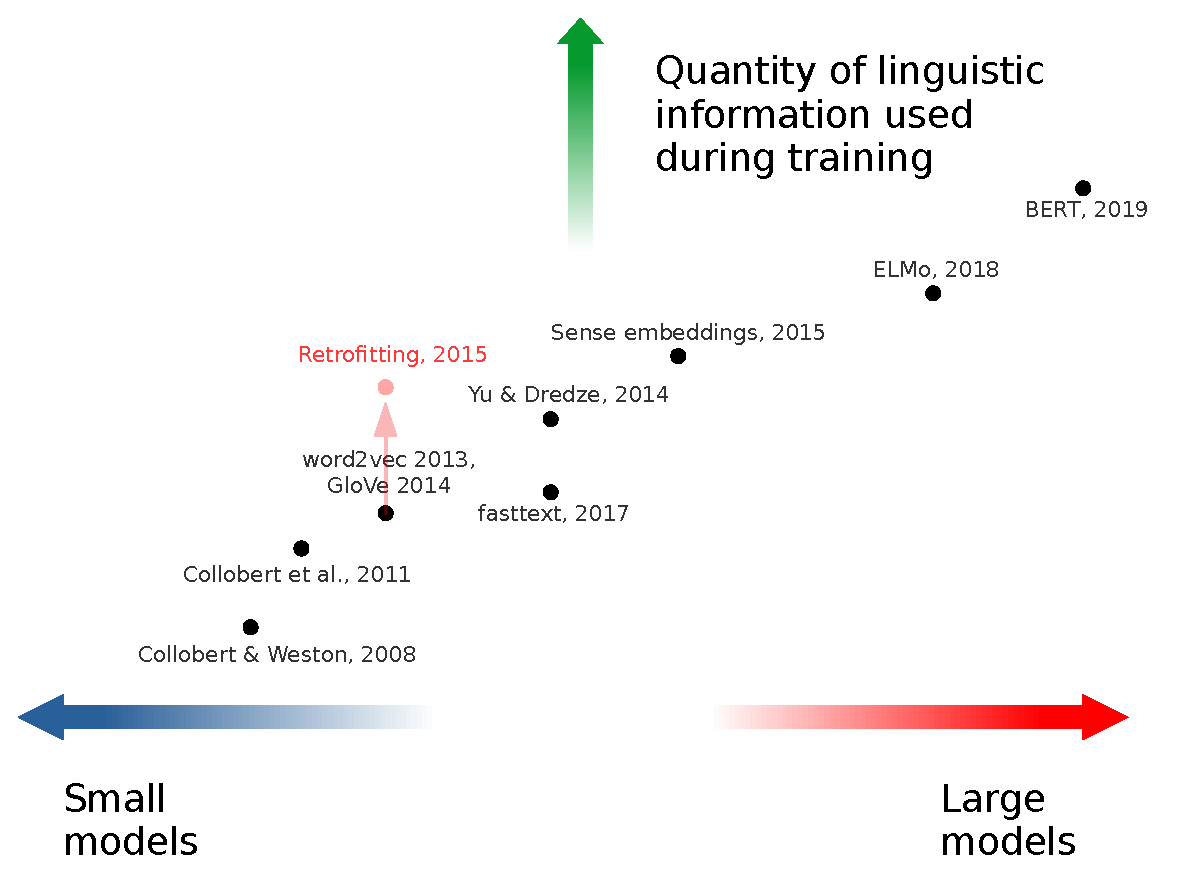
\includegraphics[width=\textwidth]{ch03-overview-WE-models}
      \caption[Visual representations of methods to learn word embeddings.]
      {Visual representations of methods to learn word embeddings. Methods on
      the left of the image generally use small architectures while the
      architecture is larger for methods placed on the right of the image. The
      vertical axis indicates on a relative scale how much information is used
      to learn word embeddings in each method.}
      \label{ch03:fig:overview-methods}
    \end{figure}

  \subsection{Strengths and weaknesses of methods to learn word embeddings}
    Methods presented in this chapter are very different in their learning
    architecture, in their training method or in the data they use. While each
    method has its own advantages and inconvenients, there exist common
    criteria to compare methods and know what are the strengths and weaknesses
    of each one. Properties of different methods are reported
    in~\autoref{ch03:tab:strength-methods}, according to four criteria:

    \begin{itemize}
      \item How much information is extracted and used from the training text
        corpus?
      \item How much information from external sources of knowledge is used
        during the training of the model?
      \item How long does it take to train the model?
      \item How large is the model architecture used by the method?
    \end{itemize}

    \noindent The strength of one method is represented by its number or
    ``\texttt{+}'' signs where more signs means a greater strength. Minus signs
    ``\texttt{-}'' indicate weaknesses where a large number of signs indicates a
    strong weakness. The number of signs is not based on any objective measure
    but is the result of my personal view and opinion on each one of those
    methods.

    \begin{table}[h]
      \centering
      \resizebox{\textwidth}{!}{
      \begin{tabular}{rcccc}
        \toprule
        & Use text corpus & Use external knowledge & Training time
        & Model size\\
        \midrule
        \citet{collobert2008unified}  & \texttt{+}    & n/a         &
                                        \texttt{++}   & \texttt{++}\\
        \citet{collobert2011natural}  & \texttt{++}   & n/a         &
                                        \texttt{+}    & \texttt{++}\\
        \texttt{word2vec} [2013]      & \texttt{++}   & n/a         &
                                        \texttt{+}    & \texttt{+}\\
        \texttt{GloVe} [2014]         & \texttt{++}   & n/a         &
                                        \texttt{+}    & \texttt{+}\\
        \texttt{fasttext} [2017]      & \texttt{+++}  & n/a         &
                                        \texttt{+}    & \texttt{-}\\
        \citet{yudredze2014improving} & \texttt{++}   & \texttt{+}  &
                                        \texttt{-}    & \texttt{+}\\
        \citet{kiela2015specializing} & \texttt{++}   & \texttt{++} &
                                        \texttt{-}    & \texttt{+}\\
        \texttt{retrofitting} [2015]  & n/a           & \texttt{++} &
                                        \texttt{+++}  & \texttt{++}\\
        Sense embeddings [2015]       & \texttt{++}   & \texttt{+}  &
                                        \texttt{-}    & \texttt{-}\\
        \texttt{ELMo} [2018]          & \texttt{++++} & n/a         &
                                        \texttt{---}  & \texttt{---}\\
        \texttt{BERT} [2019]          & \texttt{++++} & n/a         &
                                        \texttt{----} & \texttt{----}\\
      \bottomrule
      \end{tabular}}
      \caption[Strengths and weaknesses of methods to learn word
      embeddings.]{Strengths and weaknesses of different methods to learn word
      embeddings. For each criteria, the strength or weakness of one model is
      represented with plus (\texttt{+}) or minus (\texttt{-}) signs. Most of
      the values in the ``Use external knowledge'' column are set to n/a because
      most of the methods do not use external knowledge during training.}
      \label{ch03:tab:strength-methods}
    \end{table}

    Like in~\autoref{ch03:fig:overview-methods}, similar methods have similar
    properties. \citeauthor{collobert2008unified} \citep{collobert2008unified}
    use only cooccurrence information from windows of words and learn
    representations with a single hidden layer neural network. Their model is
    relatively small and fast to train because
    in~\citeyear{collobert2008unified}, training corpora were not as big as the
    ones used now and the number of parameters in their neural network is small.
    \citeauthor{collobert2011natural} \citep{collobert2011natural} extend this
    approach by using complete sentences as inputs in the neural network
    architecture instead of only using windows of words. This allows to capture
    more linguistic information in word embeddings because longer cooccurrence
    relations are used but it takes a bit longer to train the model.
    \texttt{word2vec} and \texttt{GloVe} are similar because they both use
    cooccurrence information from the text but they are trained on larger text
    corpus, so the additional information they get about rare words (which are
    usually not found in small corpus) is traded for a longer training time.
    Moreover, their model is bigger than the one used
    in~\citep{collobert2008unified, collobert2011natural} because the size of
    the vocabulary is largely increased as the size of the corpus is bigger. So
    the number of word embeddings to store during the training phase is also
    largely increased. \texttt{fasttext} has the advantage of using more
    information from the text corpus by considering morphological information
    with subwords, but it increases the model size because it needs to also
    learn one embedding per subword in addition to learning the embeddings of
    words. \medskip

    Methods which use additional external sources of
    information~\citep{yudredze2014improving, kiela2015specializing} use the
    same information from the text corpus (cooccurrence relations) as
    \texttt{word2vec} but they are slower to train because of the additional
    information used during training.~\citet{kiela2015specializing} has the
    advantage of using multiple external sources of knowledge, not a single one
    like in~\citet{yudredze2014improving}. \texttt{retrofitting} is not a
    learning method but a post-training step so it does not have to iterate over
    a large text corpus to improve word embeddings and is therefore fast to use.
    It also uses several sources of external knowledge
    like~\citet{kiela2015specializing}. Sense
    embeddings~\citep{iacobacci2015sensembed} use additional information to
    perform word disambiguation but it makes the model bigger and longer to
    train as the embeddings for each sense of each word have to be learned.
    \medskip

    Deep learning models like \texttt{ELMo} or \texttt{BERT} use bidirectional
    LSTM or transformers which are able to capture relations between words that
    are far apart from each other or that have complex context dependencies.
    Compared to models like \texttt{word2vec} or \texttt{GloVe}, they use much
    more information from the training corpus, which is one great strength of
    these approaches. Word representations learned by \texttt{ELMo} or
    \texttt{BERT} contain a lot of encoded linguistic information and the
    performances of models which use them in downstream tasks are largely
    increased. However, their model architecture is large and complex.
    \texttt{ELMo} uses 2 layers of bidirectional LSTM while \texttt{BERT} has an
    even deeper architecture with 12 layers of transformers. The number of
    computations happening inside bi-LSTM or transformers is also much greater
    than for a single hidden layer neural network. This has the consequence of
    making these models much slower to train. The computational cost of
    \texttt{ELMo} or \texttt{BERT} is a strong weakness of these approaches
    because it is difficult to replicate or to use them especially when
    computing resources are limited. \medskip

    All the presented methods have their own strengths and weaknesses. While
    simple models can be fast to train, they do not use a lot of linguistic
    information during training. Additional knowledge can be added into
    models to increase the quantity of encoded information (either with external
    sources of knowledge or by considering subwords or longer contexts) but
    using too much additional information can lead to large model architectures
    that are difficult to train because they require a lot of computing power or
    long training times. To learn word embeddings, one would have to make a
    choice between having a model that can capture a lot of linguistic
    information and having a model fast to train. A good trade-off would be to
    have a model that uses information from the text corpus with cooccurrences
    relations like in \texttt{word2vec} and which also incorporates knowledge
    from an external source of information but without adding any hard
    computational overhead so the model is still fast to train. One contribution
    of this thesis is a novel model to learn word embeddings which answers those
    requirements (see~\autoref{chap:dict2vec}).

\section{Conclusion}
  In this chapter, we have presented common methods to learn word embeddings,
  and described their main respective strengths and weaknesses.\medskip

  Basic methods use a sliding context window across a corpus to extract
  cooccurrence information between words, and update their corresponding word
  embeddings with a single hidden layer neural
  network~\citep{collobert2008unified, collobert2011natural,
  mikolov2013efficient, mikolov2013distributed}. These methods have demonstrated
  the usefulness of learning word vectors to represent linguistic properties of
  words and the impact that good representations can have when they are used in
  downstream models to solve NLP tasks. However, these methods are only based on
  the cooccurrence information of words in texts to learn word embeddings.
  Specific linguistic knowledge like synonymy is usually not found in training
  corpus and therefore is not captured by the model and incorporated into the
  embeddings.\medskip

  To overcome this shortcoming, several other approaches have been proposed to
  use additional information during training.~\citet{bojanowski2016enriching}
  use subword information while \citet{yudredze2014improving}
  and~\citet{kiela2015specializing} use external sources of knowledge to get
  information about words like hypernyms or synonyms. Additional information is
  then incorporated into a model like the \texttt{word2vec} Skip-gram model.
  Learned word representations are able to capture this additional linguistic
  information, which is beneficial for downstream models that use them because
  their performances on NLP tasks is improved compared to models that use basic
  word vectors learned from a classic \texttt{word2vec} model.\medskip

  More recent approaches use deep model architectures to learn word
  representations with either multiple bidirectional LSTM
  layers~\citep{peters2018elmo} or multi-layer
  transformers~\citep{devlin2019bert}. These models have the advantage of
  computing contextual word representations: a word is no longer associated to a
  single fixed word vector like in the \texttt{word2vec} model but a unique
  vector for each word occurrence is computed by the deep architecture depending
  on the context in which the word occurs. This approach is closer to what
  happens in a language since the meaning of a word can vary depending on its
  context. This has been observed in practice as the results on downstream tasks
  have been largely improved when models use those contextual word
  representations. However, their uses come with a rather expensive price to
  pay. Deep architectures use a lot of computations to train but also to produce
  contextual word embeddings so it greatly reduces their uses on devices with
  limited computing resources. This is an important problem as the applications
  using word embeddings are more and more used on those types of low-resource
  devices in order to off-load server-side computations or run applications
  offline.\medskip

  Two opposite strategies seem to stand out: models that use basic linguistic
  information like word cooccurrences are simple but lack some information in
  their learned representations while models that embed large quantity of
  linguistic information have richer word representations but use large
  architectures which are usually not able to run on low-resource devices. One
  may then wonder if the best parts of the two strategies can be combined, that
  is: is it possible to create a model that use large quantity of information
  during training but is small enough to be used on low-resource devices? While
  such a model is yet to be found, there exist some methods to reduce the size
  and the complexity of large models so they can be used and run on low-resource
  devices. The next chapter provides on overview of these methods.
